%-----------------------------------------------------------------------------%
\chapter{\babDua}
%-----------------------------------------------------------------------------%
Pada bab ini menjelaskan tentang tinjauan pustaka yang digunakan sebagai landasan penelitian.
Penjelasan tersebut antara lain mengenai \f{Human-Computer Interaction}, \f{user experience}, \f{e-government},
\f{usability}, \f{usability testing}, \f{prototyping} serta \f{website} Direktorat Jenderal Pajak Indonesia dan India.
%-----------------------------------------------------------------------------%

\section{\f{Human Computer Interaction}}
\f{Human Computer Interaction} (HCI) adalah bidang dalam ilmu komputer yang mempelajari bagian desain sistem yang berinteraksi langsung dengan pengguna. Ilmu ini berkembang dari kebutuhan dalam pemahaman terkait kemudahan dan kenyamanan menggunakan suatu produk perangkat lunak oleh pengguna. HCI sendiri dibagi ke dalam 2 aspek, yaitu \f{functionality} dan \f{usability} \citep{paper.mathew}. 
%-----------------------------------------------------------------------------%
\subsection{\f{Usability}}\label{subsec:usability}
\f{Usability} adalah kualitas yang menjadi penilaian bagaimana suatu tampilan antarmuka sistem dapat dengan mudah digunakan. \f{Usability} merupakan salah satu faktor penting dalam kesuksesan sitem komputer atau layanan berbasis komputer \citep{paper.smith}. Menurut (ISO/DIS 9241-11; European Usability Centre) \f{usability} menekankan kemudahan sistem untuk digunakan sesuai dengan tujuan sistem tersebut. Seperti membuat penambahan halaman pada dokumen, pengguna harus mengetaui dengan jelas apa yang perlu dilakukan serta melakukan aksi yang tidak banyak untuk mencapainya.
Banyak sekali definisi terkait dengan \f{usability} ini, namun bisa diketahui bahwa \f{usability} berkaitan erat dengan produk atau sistem dan peforma pengguna yang meliputi efektivitas, efisiensi, kemudahan dalam penggunaan serta pengalaman pengguna terkait produk atau sistem tersebut.
\newline\\
\citet{article.5ux} mengemukakan bahwa terdapat 5 komponen utama terkait \f{usability} yang mudah digunakan pengguna atau disebut juga sebagai kategori \f{user friendly}. Berikut penjabaran terkait 5 komponen utama \f{usability}, yaitu:
\pagebreak
\begin{enumerate}
	\item \f{Learnability}\\
	\f{Learnability} menjelaskan seberapa mudah aplikasi untuk dipelajari, dimengerti dan dipahami oleh pengguna ketika menggunakan produk pertama kali.
	\item \f{Efficiency}\\
	\f{Efficiency} merupakan komponen yang berkaitan dengan efisiensi menu-menu pada produk aplikasi sehingga pengguna dapat menggunakan produk secara cepat dan mudah.
	\item \f{Memorability}\\
	\f{Memorability} menjelaskan mengenai kemudahan pengguna untuk mengingat fungsi-fungsi yang terdapat pada produk aplikasi. Komponen \f{memorability} menjelaskan bahwa jika pengguna tidak menggunakan produk aplikasi dalam beberapa waktu maka ketika pengguna menggunakan produk aplikasi dapat dengan mudah menggunakannya tanpa mempelajari kembali produk aplikasi tersebut.
	\item \f{Error}\\
	\f{Error} merupakan kesalahan atau error yang dilakukan oleh pengguna ketika menggunakan produk sehingga pengguna dapat memperbaiki kesalahannya.
	\item \f{Satisfaction}\\
	\f{Satisfaction} merupakan tingkat kepuasan pengguna terhadap tampilan antarmuka dari produk aplikasi.
\end{enumerate}
Selain komponen yang dikemukakan \citeauthor{article.5ux} diatas, terdapat juga pendapat lainnya mengenai komponen \f{usability}, seperti \citet{buku.shackel} yang mengemukakan terdapat 4 komponen dalam \f{usability} antara lain \f{learnability, throughout, flexibility} dan \f{attitude}. Sementara itu \citet{paper.smith} mengemukakan bahwa \f{usability} memiliki fokus terhadap 3 komponen, yaitu \f{easy to learn, easy to use} dan kepuasan pengguna terhadap penggunaan sistem.
%-----------------------------------------------------------------------------%
\subsection{\f{User Experience}}\label{subsec:userexperience}
\f{User experience} atau disingkat UX merupakan salah satu aspek penting dalam mengembangkan suatu produk. Ilmu terkait UX sendiri sudah berkembang dari pertengahan tahun 1990-an. Interaksi antara pengguna dengan produk merupakan salah satu cakupan dari aspek UX. Definisi \f{User Experience} menurut ISO 9241-210 adalah perspektif seseorang terhadap penggunaan dari suatu produk, sistem atau layanan \citep{buku.alsos}. Sementara itu menurut \citet{article.nielsen} \f{User Experience} adalah kepuasan secara menyeluruh seorang pengguna dari hasil interaksi dengan sebuah produk atau alat digital. \citet{buku.rubin} menyebutkan bahwa \f{user experience} adalah pengalaman yang diciptakan oleh produk kepada pengguna yang menggunakannya di dunia nyata.
Terdapat beberapa definisi mengenai \f{User Experience}, namun semua rujukan tersebut menuju sebuah tujuan yaitu pengalaman pengguna terhadap penggunaan suatu produk, dengan artian produk apapun tanpa terkecuali sistem aplikasi baik berbentuk \f{website} ataupun \f{desktop}.
\newline\\
\citet{article.peter} menjelaskan dalam artikel yang berjudul "User Experience Design" bahwa UX terbagi menjadi 7 aspek. Ketujuh aspek tersebut adalah sebagai berikut.
\begin{enumerate}
	\item \f{Useful}, yaitu bermanfaat bagi pengguna.
	\item \f{Usable}, yaitu dapat dengan mudah digunakan pengguna.
	\item \f{Desireable}, yaitu memiliki elemen desain yang membangkitkan emosi dan apresiasi pengguna.
	\item \f{Findable}, yaitu kemudahan dalam pencarian konten aplikasi.
	\item \f{Accessible}, yaitu konten aplikasi dapat dengan mudah diakses pengguna. 
	\item \f{Credible}, yaitu konten aplikasi harus terpercaya.
	\item \f{Valuable}, yaitu memiliki nilai yang memenuhi dan meningkatkan kepuasan pengguna.
\end{enumerate}
%-----------------------------------------------------------------------------%
\subsection{\f{Nielsen's Usability Heuristics}}\label{subsec:nush}
\citet{article.nielsen} mengemukakan 10 prinsip terkait desain interaksi. Kesepuluh prinsip tersebut merupakan \f{usability} "\f{heuristic}" karena berbentuk aturan yang luas dan praktis serta bukan pedoman spesifik terkait \f{usability}. Kesepuluh \f{usability} heuristic tersebut, yaitu:
\begin{enumerate}
	\item \f{Visibility of system status}\\
	\f{Visibility of system status} menjelaskan mengenai sistem yang harusnya selalu menginformasikan kepada pengguna terkait apa yang terjadi melalui \f{feedback} dalam rentang waktu yang rasional kepada pengguna.
	\item \f{Match between system and the real world}\\
	\f{Match between system and the real world} menjelaskan bahwa sistem harus berkomunikasi menggunakan bahasa yang umum digunakan pengguna melalui kata, frase dan konsep yang familiar dengan pengguna daripada menggunakan tatanan bahasa yang lebih berorientasi kepada sistem. Sistem mengikuti aturan penulisan dunia nyata, membuat informasi tampil lebih natural dan tersusun secara logika.
	\item \f{User control and freedom}\\
	\f{User control and freedom} menjelaskan bahwa pengguna kadang melakukan kesalahan pada sistem sehingga membutuhkan bantuan untuk keluar dari keadaan yang tidak diinginkan tersebut tanpa berurusan dengan dialog yang panjang. Maka sistem membutuhkan fungsi yang dapat menjadi jalan keluar sehingga kesalahan tersebut dapat dihindari atau dicegah. Fitur undo dan redo merupakan salah satu contohnya.
	\item \f{Consistency and standards}\\
	\f{Consistency and standards} menjelaskan bahwa sistem harus konsisten dalam menyajikan kata karena dituasi dan aksi mengandung makna yang sama dalam sistem. Hal ini membuat pengguna tidak harus menghiraukan perbedaan dalam sistem karena sudah distandarisasi.
	\item \f{Error prevention}\\
	\f{Error prevention} menjelaskan mengenai sistem yang dapat mencegah aksi yang membuat kesalahan atau masalah dalam sistem, baik itu dengan menghilangkan kemungkinan kondisi error atau memeriksa aksi yang dilakukan pengguna dengan melakukan pertanyaan konfirmasi apa yang akan dilakukan sebelum pengguna menyetujui aksinya melalui antarmuka, karena mencegah error lebih baik daripada pesan error.
	\item \f{Recognition rather than recall}\\
	\f{Recognition rather than recall} menerangkan bahwa sistem harus dapat meminimalisir \f{memory load} pengguna dengan membuat objek, kata dan opsi yang tersedia. Dengan kata lain, pengguna tidak harus mengingat informasi dari sebuah bagian dialog ke bagian lainnya, namun instruksi penggunaan dari sistem harus mudah didapat kapanpun dibutuhkan dan dipahami pengguna.
	\item \f{Flexibility and efficiency of use}\\
	\f{Flexibility and efficiency of use} menjelaskan mengenai sistem yang dapat memberikan kemudahan dan mempercepat interaksi bagi pengguna yang tidak berpengalaman maupun berpengalaman.
	\item \f{Aesthetic and minimalist design}\\
	\f{Aesthetic and minimalist design} menjelaskan terkait estetika antarmuka yang sederhana dan indah pada sistem. Juga dijelaskan bahwa sistem harusnya tidak memiliki dialog berlebihan yang tak berkaitan sama sekali dengan tujuan sistem serta tidak dibutuhkan. 
	\item \f{Help users recognize, diagnose and recover from errors}\\
	\f{Help users recognize, diagnose and recover from errors} menjelaskan sistem harusnya memberikan pesan \f{error} kepada pengguna yang dijelaskan dengan bahasa mudah (bukan kode) dan mengindikasikan kesalahan dengan tepat serta memberikan sugesti solusi untuk menyelesaikan masalah tersebut.
	\item \f{Help and documentation}\\
	\f{Help and documentation} menjelaskan sistem yang seharusnya mudah digunakan tanpa dokumentasi tambahan, namun lebih baik jika menyediakan bantuan dan dokumentasi sehingga membantu pengguna jika mengalami kesulitan terkait fitur-fitur sistem.
\end{enumerate}
%-----------------------------------------------------------------------------%
\section{\f{Usability Testing}}\label{subsec:ust}
\f{Usability testing} merupakan sebuah metode yang digunakan untuk mengevaluasi produk/sistem yang dilakukan oleh pengguna. \citet{article.nielsen} menjelaskan bahwa \f{usability testing} merupakan metode \f{usability} yang fundamental dan tak dapat digantikan karena hal ini merupakan satu mekanisme yang mengizinkan peneliti untuk mendapatkan data dan informasi secara langsung terkait \f{user experience} suatu produk/sistem yang diujikan kepada pengguna.
\newline\\
\f{Usability testing} memiliki beberapa karakteristik secara umum. Berikut adalah karakteristik \f{usability} testing menurut \citet{buku.dumas}.
\begin{enumerate}
	\item Responden merepresentasikan target pengguna produk yang diuji. \f{Usability testing} membutuhkan responden yang berkarakteristik sama dengan pengguna target produk sesungguhnya agar produk dapat berkembang. 
	\item Responden memberikan \f{feedback} dari hasil pengerjaan tugas yang berkaitan dengan fitur-fitur utama dari produk yang diuji.
	\item Observasi dilakukan penguji kepada responden yang melaksanakan tugas yang diberikan.
	\item Dilakukan analisis data, mendaftarkan masalah dan memberikan rekomendasi solusi.
\end{enumerate}
\f{Usability testing} bertujuan untuk meningkatkan \f{usability} suatu produk sehingga berguna untuk membantu mengembangkan produk dan memastikan produk yang dikembangkan mudah dipelajari pengguna, efisien dan nyaman digunakan \citep{buku.rubin}.
\newline\\
Pengukuran \ust \space dilakukan dengan mengujikan sistem pertama kali kepada responden sehingga diperoleh penilaian pengalaman pertama pengujian dari responden \citep{buku.rubin}. Berikut merupakan komponen instrumen yang diukur dalam penilaian \ust \space milik \citeauthor{article.nielsen2} yang telah dimodifikasi \citep{paper.alotaibi}.
\begin{enumerate}
	\item Pengukuran komponen \f{usability heuristic}\\
	Pengukuran komponen \f{usability heuristic} bersifat subjektif disebabkan hasil yang dipengaruhi dari responden saat melakukan pengujian. Hal ini diamati melalui hasil kuesioner responden.
	\item Pengukuran komponen tingkat kepuasan pengguna\\
	Pengukuran dilakukan dengan memberikan pertanyaan terkait kepuasan pengguna pada instrumen penelitian.
	\item Pengukuran komponen \f{g-quality}\\
	Pengukuran komponen ini sama halnya seperti pengukuran komponen \f{usability heuristic}. Nilai yang dihasilkan tergantung dari responden saat melakukan pengujian terhadap sistem yang diujikan.
	\item Pengukuran efisiensi pengerjaan\\
	Pengukuran dilakukan dengan menghitung lama waktu pengerjaan responden ketika melakukan pengujian.  
	\item Pengukuran efektivitas pengerjaan\\
	Pengukuran efektivitas dilakukan dengan melakukan penghitungan terhadap tugas yang berhasil dikerjakan saat pengujian.
	\item Pengukuran kesalahan yan dilakukan\\
	Pengukuran kesalahan dihitung dari jumlah kesalahan responden pada saat pengujian pertama kali.
\end{enumerate}

%-----------------------------------------------------------------------------%
\section{\f{E-Government}}
\f{E-government} merupakan bagian penting dari perkembangan teknologi pemerintahan suatu negara. \f{E-government} didefinisikan sebagai pemanfaatan fasilitas \f{Internet} dan \f{World Wide Web} untuk menyampaikan informasi dan layanan pemerintahan kepada masyarakat \citep{buku.un}. \citet{paper.yen} berpendapat bahwa \f{e-government} adalah penggunaan komputer dan \f{website} sebagai sebuah media komunikasi antara pemerintah dan masyarakat.
\newline\\
\f{E-government} memiliki tugas dasar untuk memberikan layanan informasi kepada sesama istitusi pemerintah (\f{Government to Government} - G2G), dunia bisnis (\f{Government to Business} - G2B) dan kepada masyarakat (\f{Government to Citizen} - G2C) dengan tujuan sebagai berikut \citep{buku.hasibua}.
\begin{enumerate}
	\item Memberikan informasi lengkap untuk kemajuan dan peningkatan efektivitas dan produktivitas.
	\item Mampu mengoptimalkan penggunaan sumberdaya seperti waktu, tenaga, budget dan fasilitas lainnya untuk peningkatan efisiensi.
\end{enumerate}
%-----------------------------------------------------------------------------%
\subsection{Metode \f{g-Quality}}\label{subsec:gquality}
Metode \f{g-Quality} diimplementasikan oleh 7 orang spesialis pasca sarjana di bidang ilmu komputer \f{Universidade Federal Fluminense}. \citet{paper.garcia} mengemukakan dalam artikel ilmiah yang berjudul "\f{A Quality Inspection Method to Evaluate EGovernment Sites: Electrionic Government}" bahwa untuk mengevaluasi \f{website} pemerintah \f{(web based e-government)} dapat menggunakan pendekatan masyarakat sebagai fokus utama dan merealisasikan heuristic yang dibagi menjadi 5 kriteria sebagai berikut.
\begin{enumerate}
	\item \f{Cognitive Effort}, bermaksud sebagai perhatian seseorang untuk memahami dan mempelajari sebuah \f{task}. Hal ini dilakukan dengan cara meminimalisir \f{cognitive effort}, pengguna akan menjalankan \f{task} secara \f{intuitive} sehingga mencapai tujuan dengan lebih efisien. 
	\item \f{Tolerance}, merupakan motivasi dan kesabaran masyarakat dalam menunggu, memahami dan menjalankan \f{task} sesuai dengan respon website.
	\item \f{Reach}, dapat diartikan sebagai kemungkinan untuk mencapai masyarakat luas, apapun fitur teknis yang digunakan pengguna atau kemampuan spesial serta kebutuhan kognitifnya. 
	\item \f{Physical effort}, berarti kemudahan untuk menggunakan \f{website}sebagai hasil dari penggunaan data pengguna.
	\item \f{Trust}, merupakan pengujian reliabilitas dan kredibilitas, menjamin keamanan pada setiap pertukaran informasi dalam navigasi website.
\end{enumerate}
Dari kelima dasar kriteria di atas \citet{paper.garcia} mengembangkan kriteria tersebut kedalam komponen g-quality dan menambahkannya pada komponen \f{usability heuristic} milik \citeauthor{article.nielsen} untuk mengevaluasi \f{website} \f{e-government} dengan tambahan komponen sebagai berikut.
\begin{enumerate}
	\item \f{Accessibility}, bagian ini menjelaskan mengenai bagaimana sebuah \f{website} \f{e-government} dapat diraih semua kalangan, terlebih lagi orang berkebutuhan khusus.
	\item \f{Interoperability}, bagian ini menjelaskan bahwa sebuah \f{website} \f{e-government} harus dapat bertukar informasi dan layanan terhadap \f{website} \f{e-government} lainnya dengan protokol dan standar yang telah ditetapkan.
	\item \f{Security and privacy}, bagian ini menjelaskan \f{website} \f{e-government} harus terlindung dari serangan \f{hackers}, karena masyarakat akan sangat bergantung akan informasi yang disediakan. Tambahan lainnya, informasi masyarakat harus terlindungi ketika mengirimkan informasi kepada \f{website} \f{e-government}.
	\item Information truth and precision, bagian ini menjelaskan mengenai informasi yang disampaikan oleh \f{website} \f{e-government} harus benar dan tepat karena akan mempengaruhi kehidupan masyarakat. Pemerintah bertanggung jawab terhadap perawatan, perbaikan dan update dari \f{website} \f{e-government}.
	\item \f{Service agility}, bagian ini menjelaskan waktu respon terhadap permintaan masyarakat, hal ini fundamental untuk menciptakan kepercayaan dari masyarakat.
	\item \f{Transparency}, bagian ini berarti bahwa pemerintahan harus dapat membuat ketersediaan informasi publik terkait pengeluaran yang digunakan sehingga masyarakat dapat melihat dengan jelas kegiatan yang dilakukan oleh pemerintah. 
\end{enumerate} 
Dari tambahan tersebut maka penilaian \f{g-quality} digabungkan dengan \f{usability heuristic} sehingga terjadi pemetaan terhadap lima kriteria dasar pendekatan \f{e-government} kepada masyarakat. Tabel \ref{tab:mappingegov} menjelaskan hubungan kriteria terhadap \f{usability heuristic} yang telah ditambahkan penilaian g-quality.
\begin{table}
	\centering
	\caption{Pemetaan kriteria \f{e-government} terhadap komponen \f{usability heuristic} dan \f{g-Quality}}
	\label{tab:mappingegov}
	\begin{tabular}{c}
		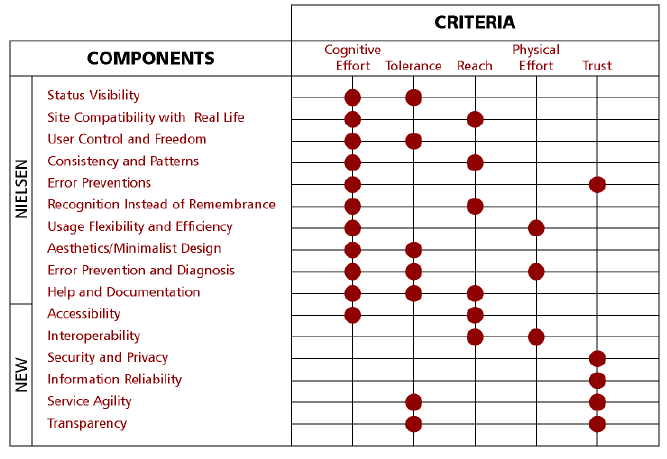
\includegraphics[width=\textwidth]
		{pics/mappinggq.PNG}
	\end{tabular}
	\begin{center}
		{\small Sumber tabel: \citep{paper.garcia}}
	\end{center}
\end{table}
%-----------------------------------------------------------------------------%
\section{\f{Prototyping}}\label{subsec:proto}
Dalam mengembangkan produk seorang pengembang pasti memerlukan gambaran ide apa yang ingin dibuat sehingga memerlukan representasi dari ide produk ke bentuk tampilan yang dapat diuji coba dan diubah seiring pengembangan. Metode gambaran proses ide produk ini biasa disebut dengan \f{prototype}. \f{Prototype} merupakan salah satu manifesto desain produk yang memungkinkan pengembang untuk berinteraksi langsung dan mengeksplorasi kesesuaiannya secara langsung \citep{buku.preece}. \f{Prototype} memiliki banyak bentuk untuk merepresentasikan suatu produk, terdapat juga \f{prototype} berdasarkan \f{outline} kertas yang merepresentasikan tampilan atau serangkaian tampilan, sebuah gambar elektronik, simulasi video atau rangkaian maket sebagai tampilan \f{mockup} keseluruhan rancangan. \f{Prototype} digunakan sebagai bantuan dalam mendiskusikan ide antar \f{stakeholders}. Schon (1983) mendeskripsikan bahwa \f{prototype} diakui oleh desainer berbagai ilmu disiplin sebagai sebuah aspek penting dalam proses desain. \f{Prototype} menurut \citet{buku.preece} terbagi menjadi dua jenis, yaitu \f{Low-Fidelity Prototyping} dan \f{High-Fidelity Prototyping}.
%-----------------------------------------------------------------------------%
\subsection{\f{Low-Fidelity Prototyping}}
\f{Low-Fidelity Prototyping} merupakan proses pengembangan desain \f{prototype} yang hasilnya tidak sama dengan produk akhir. Biasanya \f{prototyping} ini menggunakan material \f{paper-based model} atau kardus daripada menggunakan material tampilan elektronik dan metal. Metode ini sangat mudah digunakan karena simpel, cepat dan murah dalam produksinya sehingga sangat sensitif akan perubahan untuk pergantian desain atau ide. \f{Prototype} jenis ini dibuat bukan untuk disimpan dan diintegrasikan dengan produk akhir, dibuat hanya untuk penelusuran ide lebih lanjut. 
\newline\\
\f{Low-fidelity prototyping} terdiri dari dua macam, yaitu \f{storyboard} dan \f{sketch}. \f{Storyboard} merupakan metode \f{prototyping} yang menggunakan skenario dalam menjalankannya. \f{Storyboard} biasanya tersusun dari sketsa berseri yang menunjukkan bagaimana proses seorang pengguna dalam menjalankan \f{task} pada aplikasi. Gambar \ref{fig:story} menjelaskan mengenai seseorang yang menggunakan sebuah sistem baru untuk mendigitalisasi gambar (Hartfield dan Winogard, 1996).

\begin{figure}
	\centering
	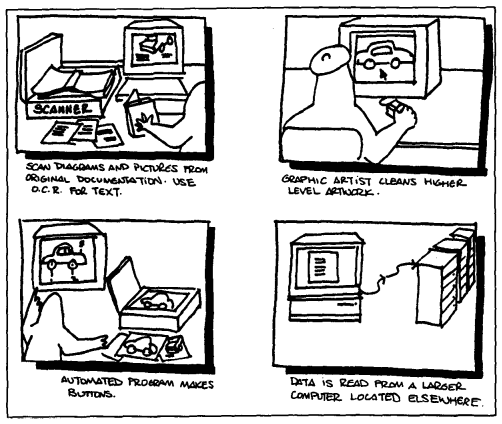
\includegraphics[width=0.8\textwidth]
	{pics/storyboard.PNG}
	\caption{\f{Storyboard} sederhana}
	\label{fig:story}
\end{figure}
\begin{center}
	{\small Sumber gambar: \citep{buku.preece}}
\end{center}
\f{Sketch} merupakan metode \f{prototyping} yang menggunakan sebuah sketsa dalam menjalankannya, penggunaan metode sketsa dianggap sulit karena banyak yang merasa kurang ahli dalam menggambar. Gambar \ref{fig:sketsa} menunjukan sebuah contoh dari sketsa sederhana.
\begin{figure}
	\centering
	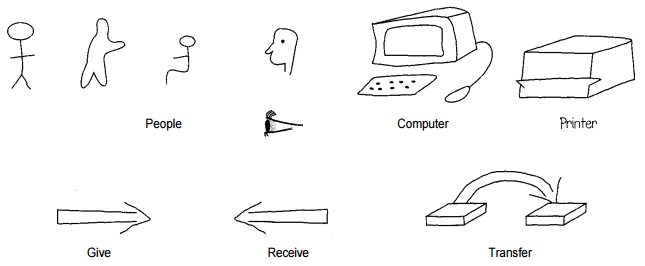
\includegraphics[width=\textwidth]
	{pics/simplesketch.PNG}
	\caption{\f{Sketch} sederhana}
	\label{fig:sketsa}
\end{figure}
\begin{center}
	{\small Sumber gambar: \citep{buku.preece}}
\end{center}
%-----------------------------------------------------------------------------%
\subsection{\f{High-Fidelity Prototyping}}
Perkembangan lebih lanjut dari \f{low-fidelity prototyping} adalah \f{high-fifelity prototyping}. \f{High-fidelity prototyping} biasa digunakan dalam pengembangan produk yang dianggap sebagai produk akhir. Proses pembuatan \f{prototype} dibuat dengan material yang diharapkan digunakan dalam produk akhir sehingga produk \f{prototype} mirip dengan aslinya. Sebagai contoh produk perangkat lunak yang dikembangkan dengan menggunakan \f{Visual Basic} memiliki kesesuaian lebih tinggi dibanding \f{paper-based mockup}. \f{High-fidelity prototyping} biasanya digunakan untuk menjual ide kepada orang lain dan percobaan terkait kendala teknis.
%-----------------------------------------------------------------------------%
\section{\f{Website} Direktorat Jenderal Pajak}
Perkembangan teknologi di bidang komunikasi menuntut pemerintah melakukan pendekatan kepada masyarakat di segala bidang pelayanan, tanpa terkecuali pada bidang perpajakan. Kebutuhan akan pelayanan perpajakan yang mulai diperbaharui mengikuti perkembangan jaman, memicu suatu negara untuk mengadakan layanan e-government. Website departemen kementrian suatu pemerintahan merupakan salah satu implementasi dari e-government secara umum. Setiap departemen memiliki ciri khasnya masing-masing. Pada bagian ini akan dijelaskan mengenai \f{website} Direktorat Jenderal Pajak Indonesia dengan India.
%-----------------------------------------------------------------------------%
\subsection{\f{Website} Direktorat Jenderal Pajak Indonesia}
\begin{figure}
	\centering
	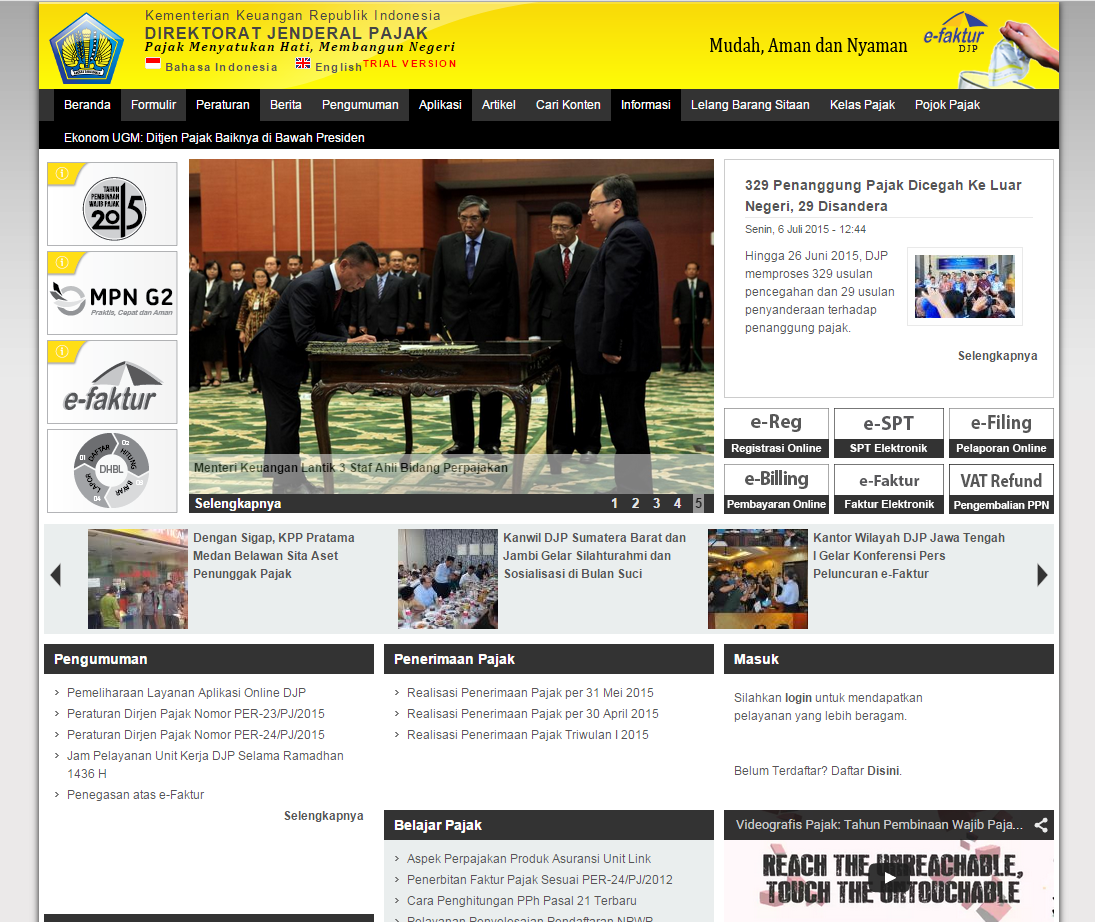
\includegraphics[width=\textwidth]
	{pics/pajakweb.PNG}
	\caption{Tampilan \f{website} Direktorat Jenderal Pajak Indonesia}
	\label{fig:pajakweb}
\end{figure}
\begin{center}
	{\small Sumber gambar: pajak.go.id}
\end{center}
Website direktorat jenderal pajak (DJP) Indonesia mulai hadir di Indonesia pada akhir 2010. Seiring dengan dikeluarkannya peraturan menteri Keuangan Nomor 184/ PMK.01/2010 tentang organisasi dan tata kerja kementerian keuangan\footnote{\url{http://www.pajak.go.id/content/selayang-pandang}}. Layanan yang tersedia di \f{website} pajak.go.id ini sendiri merupakan layanan portal yang menghubungkan informasi dari DJP dengan aplikasi perpajakan yang dimilikinya. Aplikasi perpajakan yang disediakan DJP adalah \f{e-filling, e-faktur, e-SPT, e-registration} dan \f{e-billing}. Dari kesemua aplikasi tersebut beberapa diantaranya ada yang kurang berjalan dengan maksimal. 
\newline\\
\f{E-filling} merupakan salah satu aplikasi web buatan DJP yang berjalan cukup baik dibandingkan dengan aplikasi lainnya. \f{E-filling} berfungsi sebagai form online untuk pengisian Surat Pajak Tahunan baik satuan ataupun badan. Gambar \ref{fig:pajakweb} menunjukkan tampilan beranda dari \f{website} Direktorat Jenderal Pajak Indonesia.
%-----------------------------------------------------------------------------%
\subsection{\f{Website} Direktorat Jenderal Pajak India}
\begin{figure}
	\centering
	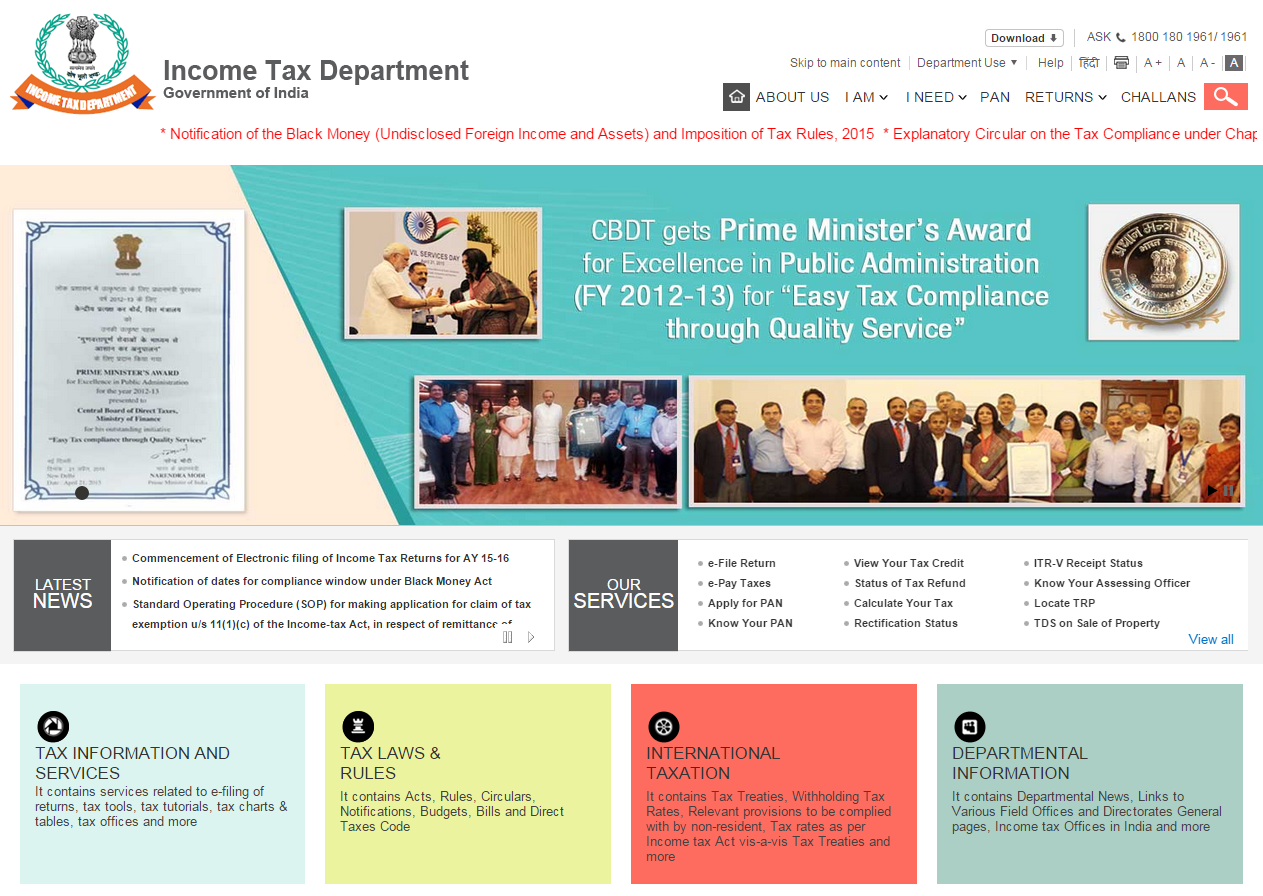
\includegraphics[width=\textwidth]
	{pics/pajakindiaweb.PNG}
	\caption{Tampilan \f{website} Direktorat Jenderal Pajak India}
	\label{fig:pajakindiaweb}
\end{figure}
\begin{center}
	{\small Sumber gambar: incometaxindia.gov.in}
\end{center}
Website Direktorat Jenderal Pajak India mulai muncul ke publik setelah India resmi membuka seluruh akses \f{e-government}-nya kepada publik. Dalam perkembangannya sendiri, \f{website} DJP India merupakan salah satu sistem \f{e-government} yang lebih dulu hadir dalam tatanan sistem besar \f{e-government} India. Sistem \f{website}pajak India didirikan sudah sejak tahun 2001\footnote{\url{http://arc.gov.in/11threp/arc_11threport_ch4.pdf}} namun digunakan dalam lingkup internal. Setelah penggunaan internal \f{website}, DJP India mengeluarkan website baru pada tahun 2014 secara umum\footnote{\url{http://www.incometaxindia.gov.in/Pages/about-us/history-of-direct-taxation.aspx}}.
\newline\\
Secara umum \f{website} DJP India menyediakan aplikasi yang tak jauh berbeda dengan \f{website} DJP Indonesia. Namun di India diterapkan sistem PAN (Personal Authentification Number) yang membuat setiap warga negara terwajib pajak dapat langsung menikmati fasilitas pelayanan \f{e-government}. Gambar \ref{fig:pajakindiaweb} menunjukkan mengenai tampilan beranda dari \f{website} Direktorat Jenderal Pajak India.
%-----------------------------------------------------------------------------%
\section{Aplikasi \f{Web} InvisionApp}\label{subsec:invisionapp}
\begin{figure}
	\centering
	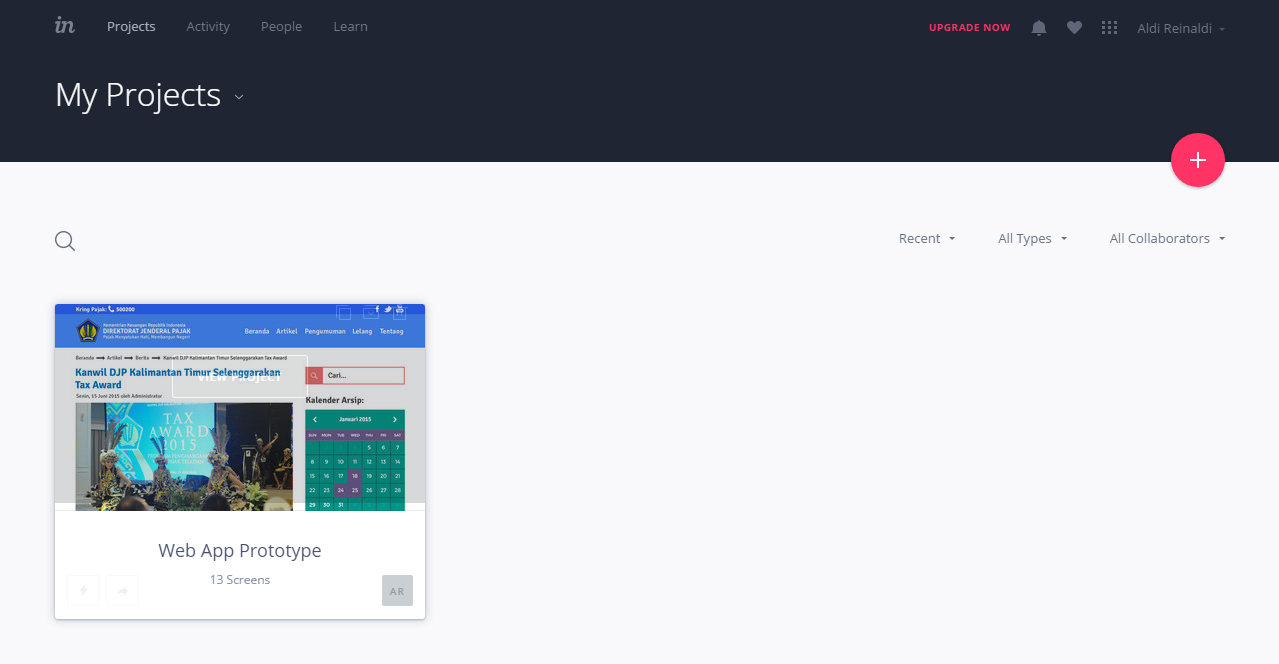
\includegraphics[width=\textwidth]
	{pics/invisionapp.PNG}
	\caption{Tampilan \f{website} InvisionApp.com}
	\label{fig:pajakindiaweb} 	
\end{figure}
\begin{center}
	{\small Sumber gambar: invisionapp.com}
\end{center}
\f{Invisionapp} adalah aplikasi berbasis \f{web} yang memberikan layanan untuk pembuatan \f{prototype} secara cepat. Aplikasi \f{web} ini memberikan pelayanan gratis untuk pelanggannya, lalu akan memberikan tawaran \f{upgrade} untuk menggunakan fitur tertentu.
\newline\\
Aplikasi \f{web} ini mengijinkan pengguna yang telah terdaftar untuk membuat \f{clickable prototype} baik itu dalam bentuk \f{prototype} \f{website} atau pun \f{prototype} aplikasi mobile. Aplikasi web ini memudahkan bagi para developer atau pun desainer untuk melihat desain \f{prototype} yang lebih hidup\footnote{\url{http://www.invisionapp.com/}}.
Gambar \ref{subsec:invisionapp} menunjukkan tampilan dari proyek yang sedang dikerjakan oleh pengguna.
%-----------------------------------------------------------------------------%